\chapter{Dual-Arm Shared Vision and Reachability-Based Role Assignment}
\label{chap:shared_vision}

Chapter~\ref{chap:vision_pipelines} developed two perception pipelines that return a bolt's pose in
a single manipulator's base frame. That is sufficient when exactly one arm is available to act on
whatever is detected. Chapter~\ref{chap:lit_review} identified gap G2 as what happens once a second
arm shares the workspace: existing coordination schemes decide which arm acts either by coupling
both arms' motion at the control level, by solving a scheduling problem from a centrally available,
typically external, view of the scene, or by dividing the workspace into static zones computed
offline. In no case is a second arm's own onboard camera used to decide, at the moment a target is
found, which arm should manipulate it~\citep{sk2025sharedvision}.

This chapter presents the dual-arm shared-vision system that closes that gap. Two 6-DOF Kinova
Gen3 Lite manipulators, each carrying its own wrist-mounted eye-in-hand camera rather than relying
on a shared external sensor, independently search a common tabletop workspace. Whichever arm's
camera detects the target first relays the detected pose into the other arm's base frame through a
calibrated inter-arm transform, so that reachability can be evaluated for both arms regardless of
which one made the detection. A runtime rule then assigns the task to whichever arm can actually
reach the target, and the selected arm executes the pick-and-place sequence under damped
least-squares resolved-rate control. Section~\ref{sec:sv_architecture} sets out the system
architecture and kinematic model. Section~\ref{sec:sv_search} covers the independent search
trajectory and visual target localization. Section~\ref{sec:sv_relay} presents the cross-frame pose
relay, and Section~\ref{sec:sv_reachability} the reachability-based role-assignment rule built on
top of it. Section~\ref{sec:sv_control} covers the manipulation sequence and the resolved-rate
control law that executes it, and Section~\ref{sec:sv_results} presents end-to-end validation in
Gazebo/ROS2 simulation and on physical dual-arm hardware.

%% ============================================================
\section{System Architecture and Kinematic Model}\label{sec:sv_architecture}
%% ============================================================

The platform consists of two Kinova Gen3 Lite manipulators, denoted $\mathcal{A}_L$ (LEFT) and
$\mathcal{A}_R$ (RIGHT), sharing a common tabletop workspace, each carrying its own wrist-mounted
eye-in-hand camera rather than a shared external sensor. Both arms first home concurrently, then
search the shared workspace while running fiducial-marker detection on their own camera stream;
once either arm's camera locates the target, its pose is relayed into both arms' own base frames,
and a reachability-based rule selects which arm proceeds to manipulate it, resuming the search if
neither arm can reach it. Figure~\ref{fig:sv_overall} summarizes the complete pipeline.

\begin{figure}[htbp]
\centering
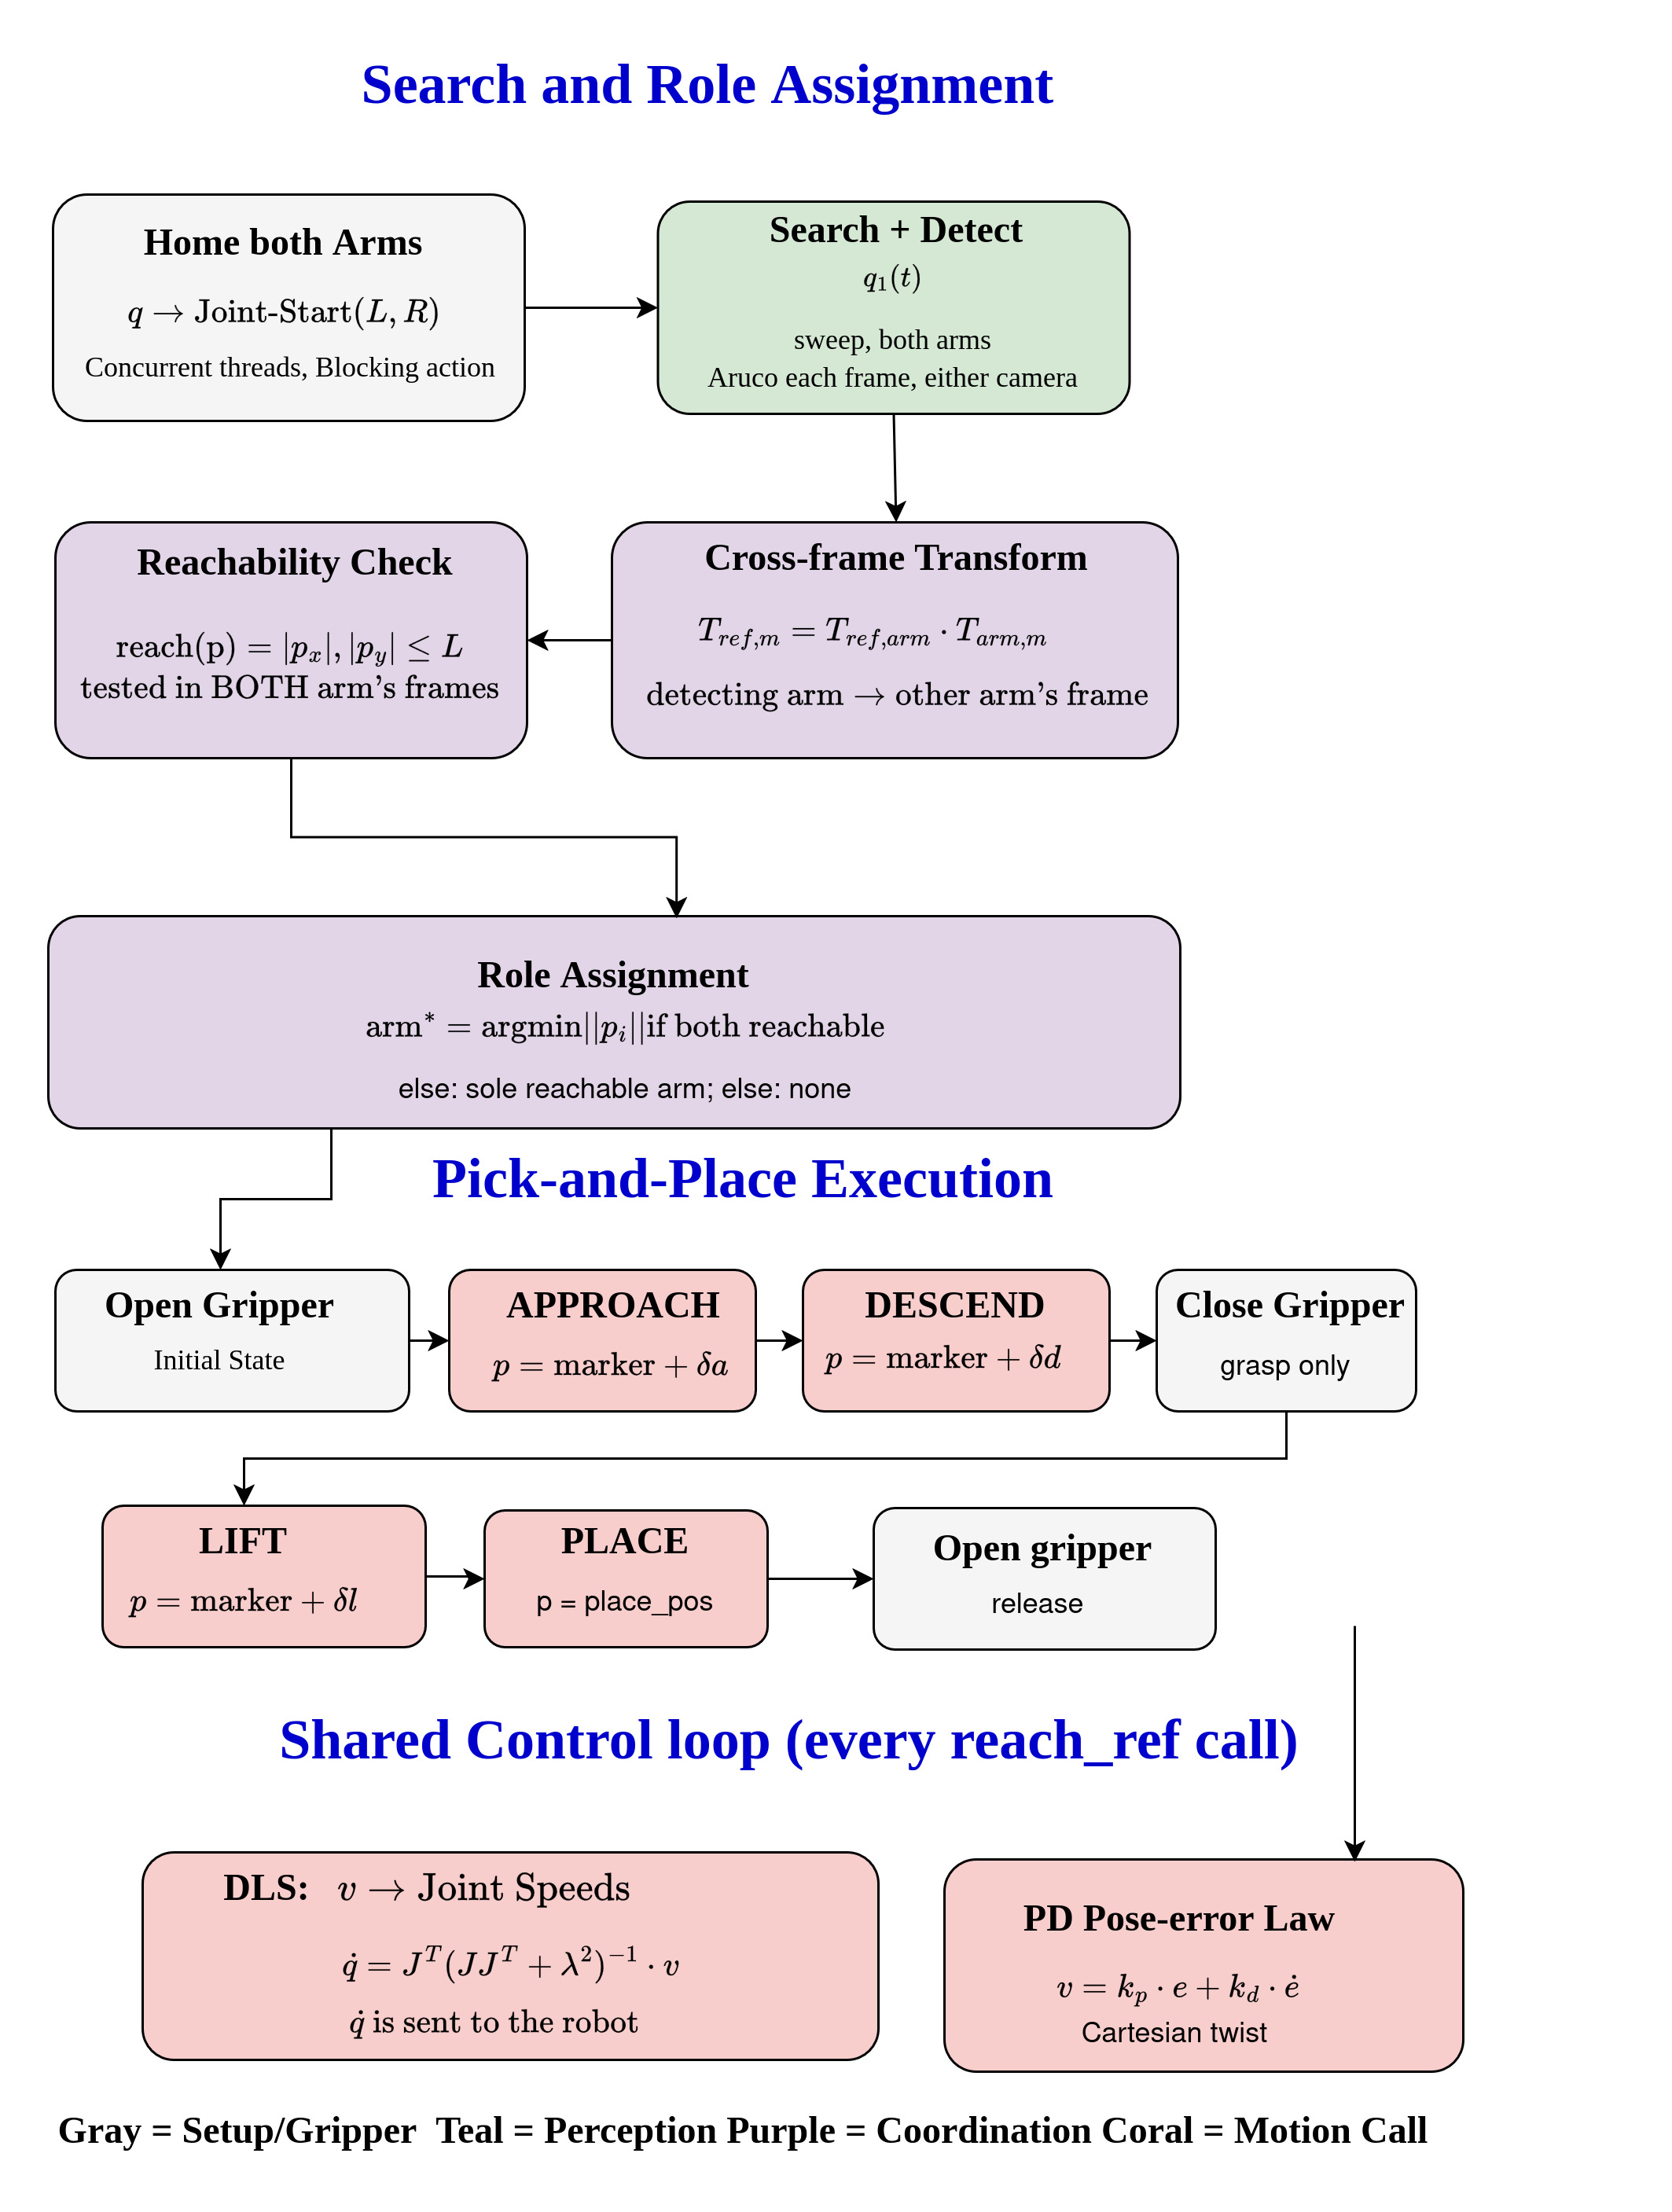
\includegraphics[width=0.85\linewidth]{Images/sharedVision/overall_architecture.jpg}
\caption{Overall architecture: concurrent homing and search, cross-frame pose relay,
reachability-based role assignment, and pick-and-place execution under the shared resolved-rate
control loop~\citep{sk2025sharedvision}.}
\label{fig:sv_overall}
\end{figure}

Each arm reuses the base frame $B$, gripper frame $G$, and camera frame $C$ convention of
Figure~\ref{fig:vp_frames}, with the camera frame now wrist-mounted rather than globally fixed, and
the bolt frame $F$ of Chapter~\ref{chap:vision_pipelines} generalized to a fiducial marker frame
$M$, since this chapter localizes an ArUco marker rather than a bolt. Because the two arms are
kinematically identical, the equations of this section apply to either arm and the arm index is
omitted; it is reintroduced in Section~\ref{sec:sv_relay}, where quantities from both arms must be
related to one another.

Each arm's forward kinematics is a chain of fixed-geometry, single-DOF homogeneous transforms
$T^{k-1}_{k}(q_k)$, where $T^{j}_{i}$ denotes, as in Equation~\eqref{eq:vp_transform}, the transform
that expresses frame $i$'s coordinates in frame $j$:
\begin{equation}
T^{B}_{6}(\mathbf{q}) = T^{B}_{1}(q_1)\,T^{1}_{2}(q_2)\,T^{2}_{3}(q_3)\,T^{3}_{4}(q_4)\,
T^{4}_{5}(q_5)\,T^{5}_{6}(q_6), \qquad \mathbf{q} = [q_1, \ldots, q_6] \in \mathbb{R}^6.
\label{eq:sv_fwdkin}
\end{equation}
Two further fixed transforms extend the chain to the gripper frame and the eye-in-hand camera
frame:
\begin{equation}
T^{B}_{G}(\mathbf{q}) = T^{B}_{6}(\mathbf{q})\,T^{6}_{G}, \qquad
T^{B}_{C}(\mathbf{q}) = T^{B}_{G}(\mathbf{q})\,T^{G}_{C},
\label{eq:sv_toolcam}
\end{equation}
where $T^{6}_{G}$ is the fixed gripper-frame offset and $T^{G}_{C}$ is the fixed eye-in-hand camera
offset, identical by construction on both arms. Unlike the fixed camera-to-base transform of
Section~\ref{sec:vp_notation}, which was calibrated once for a globally mounted camera,
$T^{B}_{C}(\mathbf{q})$ varies with the arm's own joint configuration $\mathbf{q}$ because the
camera moves with the wrist.

The manipulator Jacobian $J(\mathbf{q}) \in \mathbb{R}^{6\times 6}$ is obtained by central-difference
numerical differentiation of $T^{B}_{G}$:
\begin{equation}
J_{:,i} =
\begin{bmatrix}
\dfrac{\mathbf{p}(\mathbf{q}+\epsilon\mathbf{e}_i) - \mathbf{p}(\mathbf{q}-\epsilon\mathbf{e}_i)}{2\epsilon} \\[1.2ex]
\dfrac{\log\!\left( R(\mathbf{q}+\epsilon\mathbf{e}_i)\, R(\mathbf{q}-\epsilon\mathbf{e}_i)^\top \right)}{2\epsilon}
\end{bmatrix}, \qquad \epsilon = 10^{-6},
\label{eq:sv_jacobian}
\end{equation}
where $\mathbf{p}(\cdot)$ and $R(\cdot)$ are the translational and rotational parts of $T^{B}_{G}$
and $\mathbf{e}_i$ is the $i^{\text{th}}$ standard basis vector. The rotation term uses $R^\top$ in
place of $R^{-1}$, valid since $R^{-1} = R^\top$ for all $R \in SO(3)$. Unlike position, which lies
in a vector space and admits a direct central difference, rotations do not subtract meaningfully;
$\log(\cdot)$ denotes the matrix logarithm mapping a relative rotation
$R(\mathbf{q}+\epsilon\mathbf{e}_i)R(\mathbf{q}-\epsilon\mathbf{e}_i)^\top \in SO(3)$ to its
axis-angle vector in $\mathbb{R}^3$. Since this relative rotation accumulates over the interval
$[-\epsilon, \epsilon]$, its rotation vector is approximately $2\epsilon$ times the instantaneous
angular-velocity direction, so dividing by $2\epsilon$ recovers the angular-velocity Jacobian column
exactly as the position rows recover the linear one.

%% ============================================================
\section{Search Trajectory and Visual Target Localization}\label{sec:sv_search}
%% ============================================================

Both arms first execute a blocking angular move, in independent threads so neither arm idles
waiting for the other, to a per-arm predefined start configuration $\mathbf{q}_0^{L}, \mathbf{q}_0^{R}$.
Each arm then independently sweeps its own joint 1 at constant angular speed, reversing direction at
each bound rather than following a smooth periodic profile:
\begin{equation}
\dot{q}_1(t) =
\begin{cases}
+\dot{q}_{\text{sweep}}, & q_1(t) \leq q_1^{\max} \text{ and direction} = +1, \\
-\dot{q}_{\text{sweep}}, & q_1(t) \geq q_1^{\min} \text{ and direction} = -1,
\end{cases}
\label{eq:sv_search}
\end{equation}
with direction flipping at each bound, and bounds computed from that arm's own start angle
$q_{1,0}$, a sweep half-range $\Delta_{\text{search}}$, and the joint's hard limits
$q_1^{\text{lo}}, q_1^{\text{hi}}$ with safety margin $\epsilon_q$:
\begin{equation}
q_1^{\min} = \max\!\left( q_{1,0} - \Delta_{\text{search}},\, q_1^{\text{lo}} + \epsilon_q \right),
\qquad
q_1^{\max} = \min\!\left( q_{1,0} + \Delta_{\text{search}},\, q_1^{\text{hi}} - \epsilon_q \right).
\label{eq:sv_searchbounds}
\end{equation}
While sweeping, each arm continuously runs ArUco marker detection on its own camera
stream~\citep{garrido2014automatic}. Given a detected marker's corner correspondences, a
perspective-$n$-point (PnP) pose estimator yields the marker's pose relative to the camera,
$(\mathbf{t}_{cm}, R_{cm})$, which is assembled into the transform $T^{C}_{M}$. Using the live
camera pose $T^{B}_{C}(\mathbf{q})$ at the instant of detection, the marker pose is expressed in the
detecting arm's own base frame by the same composition rule as
Equation~\eqref{eq:vp_transform}:
\begin{equation}
T^{B}_{M} = T^{B}_{C}(\mathbf{q})\, T^{C}_{M}, \qquad
T^{C}_{M} = \begin{bmatrix} R_{cm} & \mathbf{t}_{cm} \\ \mathbf{0}^\top & 1 \end{bmatrix}.
\label{eq:sv_marker}
\end{equation}

%% ============================================================
\section{Cross-Frame Pose Relay}\label{sec:sv_relay}
%% ============================================================

The two arms' base frames are related by a fixed, calibrated rigid transform. Let $B_L$ and $B_R$
denote the LEFT and RIGHT base frames, and take $B_L$ as the shared reference frame, so that
$T^{B_L}_{B_L} = I$ and $T^{B_L}_{B_R} \in SE(3)$ is the calibrated transform expressing RIGHT-frame
coordinates in the shared reference frame (a translation of $[1.08, 0, 0]$\,m together with a
$180^\circ$ rotation about $z$, reported in Table~\ref{tab:sv_params}). A marker detected in
$a_d \in \{L, R\}$'s own base frame, $T^{B_{a_d}}_{M}$ from Equation~\eqref{eq:sv_marker}, is relayed
into the shared reference frame and then into the other arm $a_o$'s own frame by
\begin{equation}
T^{B_L}_{M} = T^{B_L}_{B_{a_d}}\, T^{B_{a_d}}_{M}, \qquad
T^{B_{a_o}}_{M} = \left( T^{B_L}_{B_{a_o}} \right)^{-1} T^{B_L}_{M}.
\label{eq:sv_relay}
\end{equation}
This round trip through the shared reference frame is what allows a target detected by one arm's
camera to be evaluated in the other arm's own frame, regardless of which arm made the detection,
without requiring a shared external sensor.

%% ============================================================
\section{Reachability-Based Role Assignment}\label{sec:sv_reachability}
%% ============================================================

Reachability of a position $\mathbf{p}$, expressed in a given arm's own base frame, is tested
against that arm's calibrated workspace half-extent $L_w$:
\begin{equation}
\operatorname{reach}(\mathbf{p}) =
\begin{cases}
1, & |p_x| \leq L_w \text{ and } |p_y| \leq L_w, \\
0, & \text{otherwise}.
\end{cases}
\label{eq:sv_reach}
\end{equation}
Upon detection, $\operatorname{reach}(\cdot)$ is evaluated for both arms using their respective
local pose from Equation~\eqref{eq:sv_relay}, and the acting arm is selected by
\begin{equation}
\text{arm}^{*} =
\begin{cases}
a_d, & \text{if only } a_d \text{ satisfies reach}, \\
a_o, & \text{if only } a_o \text{ satisfies reach}, \\
\displaystyle\arg\min_{i \in \{L, R\}} \lVert \mathbf{p}_i \rVert, & \text{if both satisfy reach}, \\
\varnothing, & \text{otherwise},
\end{cases}
\label{eq:sv_roleassign}
\end{equation}
where $a_d$ and $a_o$ are the detecting and other arm respectively, and $\mathbf{p}_i$ is the
target's position in arm $i$'s own base frame. When neither arm can reach the target, both resume
the search of Section~\ref{sec:sv_search} rather than forcing an infeasible assignment. This rule
is what removes the need for either a centrally solved allocation problem or an offline static
zoning of the workspace: reachability is decided per detection, at runtime, from pose information
each arm already has once Equation~\eqref{eq:sv_relay} has run.

\begin{table}[htbp]
\centering
\caption{System and controller parameters.}
\label{tab:sv_params}
\resizebox{\textwidth}{!}{%
\begin{tabular}{lll}
\toprule
\textbf{Symbol} & \textbf{Description} & \textbf{Value} \\
\midrule
\multicolumn{3}{l}{\textit{Kinematics and rig geometry}} \\
$\epsilon$              & Central-difference step (Equation~\eqref{eq:sv_jacobian})       & $10^{-6}$ \\
$T^{B_L}_{B_R}$          & Inter-arm transform (translation; rotation)                      & $[1.08, 0, 0]$~m; $R_z(180^\circ)$ \\
$L_w$                   & Workspace half-extent (Equation~\eqref{eq:sv_reach})             & $0.5$~m \\
\midrule
\multicolumn{3}{l}{\textit{Search trajectory}} \\
$\dot{q}_{\text{sweep}}$ & Joint-1 sweep speed                                              & $8^\circ$/s \\
$\Delta_{\text{search}}$ & Sweep half-range                                                 & $120^\circ$ \\
$\epsilon_q$             & Joint-limit safety margin                                        & $0.08$~rad \\
\midrule
\multicolumn{3}{l}{\textit{Perception}} \\
--                       & ArUco dictionary~\citep{garrido2014automatic}                      & \texttt{5X5\_50} \\
--                       & Marker side length                                               & $0.05$~m \\
\midrule
\multicolumn{3}{l}{\textit{Manipulation waypoints}} \\
$\mathbf{a}$             & Approach offset, $\mathcal{A}_L$ / $\mathcal{A}_R$               & $[.05,.02,.07]$ / $[.03,.07,.07]$~m \\
$d$                      & Descend distance                                                 & $0.08$~m \\
$l$                      & Lift height                                                      & $0.10$~m \\
\midrule
\multicolumn{3}{l}{\textit{Resolved-rate control}~\citep{whitney1969resolved}} \\
$K_p^{\text{pos}}, K_d^{\text{pos}}$ & Position PD gains                                    & $2.0$, $0.05$ \\
$K_p^{\text{ori}}, K_d^{\text{ori}}$ & Orientation PD gains                                 & $0.9$, $0.04$ \\
$\tau$                   & Derivative filter time constant                                  & $0.06$~s \\
$\lambda$                & DLS damping~\citep{chiaverini1994review} (nominal / near singular) & $0.12$ / $0.45$ \\
$\mu_{\min}$             & Manipulability switch threshold                                  & $0.01$ \\
$\dot{q}_{\max}$         & Joint-speed saturation                                           & $0.2$~rad/s \\
--                       & Control loop rate                                                & $10$~Hz \\
\midrule
\multicolumn{3}{l}{\textit{Convergence tolerances}} \\
--                       & Position / orientation, APPROACH, LIFT, PLACE                     & $8$~mm / $5^\circ$ \\
--                       & Position / orientation, DESCEND (grasp)                          & $5$~mm / $3^\circ$ \\
--                       & Consecutive cycles in tolerance                                  & $3$ \\
\bottomrule
\end{tabular}%
}
\end{table}

%% ============================================================
\section{Manipulation Sequence and Resolved-Rate Control}\label{sec:sv_control}
%% ============================================================

Once $\text{arm}^*$ is selected, it executes a seven-step sequence: open gripper; APPROACH;
DESCEND; close gripper (grasp); LIFT; PLACE; open gripper (release). Only APPROACH, DESCEND, and
LIFT are derived from the marker position $\mathbf{p}_m$ in $\text{arm}^*$'s own frame; each is
built from the previous target rather than independently offset from the marker, and grasp itself
involves no motion target:
\begin{equation}
\mathbf{p}_{\text{approach}} = \mathbf{p}_m + \mathbf{a}, \qquad
\mathbf{p}_{\text{descend}} = \mathbf{p}_{\text{approach}} - \begin{bmatrix} 0 \\ 0 \\ d \end{bmatrix}, \qquad
\mathbf{p}_{\text{lift}} = \mathbf{p}_{\text{descend}} + \begin{bmatrix} 0 \\ 0 \\ l \end{bmatrix},
\label{eq:sv_waypoints}
\end{equation}
where $\mathbf{a}$ is a fixed per-arm approach offset and $d, l$ are fixed scalar descend and lift
distances (grasp is a gripper actuation at $\mathbf{p}_{\text{descend}}$, not a fifth target). The
PLACE target $\mathbf{p}_{\text{place}}$ is, by contrast, a fixed pre-configured drop-off pose for
$\text{arm}^*$, independent of $\mathbf{p}_m$. Grasp yaw is resolved under the gripper's
$180^\circ$ symmetry by choosing, of the two equivalent orientations, whichever has the greater
quaternion alignment with the arm's current tool orientation, minimizing unnecessary wrist rotation.

%% ------------------------------------------------------------
\subsection{Damped Least-Squares Resolved-Rate Control}\label{subsec:sv_dls}
%% ------------------------------------------------------------

Every one of the four motion targets above is reached by the same control loop, extending resolved-
rate motion control~\citep{whitney1969resolved} with damping for singularity
robustness~\citep{wampler1986manipulator,chiaverini1994review,nakamura1986inverse} and with the
Cartesian pose error itself computed from the eye-in-hand visual feedback of
Section~\ref{sec:sv_search}, in the manner of classical visual servo
control~\citep{hutchinson1996tutorial}. Given position and orientation error
$(\mathbf{e}_p, \mathbf{e}_o, \theta_e)$ between the current and target tool pose, a PD law with a
first-order low-pass-filtered derivative produces a Cartesian twist $\mathbf{v}$, an intermediate
quantity rather than a robot command:
\begin{equation}
\mathbf{v} =
\begin{bmatrix}
K_p^{\text{pos}}\,\mathbf{e}_p + K_d^{\text{pos}}\,\dot{\mathbf{e}}_{p,\text{filt}} \\
K_p^{\text{ori}}\,\mathbf{e}_o + K_d^{\text{ori}}\,\dot{\mathbf{e}}_{o,\text{filt}}
\end{bmatrix}.
\label{eq:sv_twist}
\end{equation}

The filtered derivative in Eq.~\ref{eq:sv_twist} is a discrete first-order low-pass of the raw error difference, with time constant $\tau$ and control period $\Delta t$, as in Eq.~\ref{deriv_filter}:
\begin{equation}
\dot{\mathbf{e}}_{\mathrm{filt}}
\leftarrow
\alpha\,\frac{\mathbf{e}_{k}-\mathbf{e}_{k-1}}{\Delta t}
+
(1-\alpha)\,\dot{\mathbf{e}}_{\mathrm{filt}},
\qquad
\alpha=\frac{\Delta t}{\tau+\Delta t}.
\label{deriv_filter}
\end{equation}
applied independently to $\mathbf e_p$ and $\mathbf e_o$; without it, the $K_d$ terms would amplify the quantization noise of the $10$~Hz joint feedback straight into the commanded twist.


This twist is mapped to the joint speeds actually sent to the arm by damped least-squares inverse
differential kinematics:
\begin{equation}
\dot{\mathbf{q}} = J^\top \left( J J^\top + \lambda^2 I \right)^{-1} \mathbf{v},
\label{eq:sv_dls}
\end{equation}
with $\lambda$ switched between a nominal and a larger value near singularities using the
manipulability measure $\mu(\mathbf{q}) = \sqrt{\det(J J^\top)}$ as in \ref{lambda_switch}, and $\dot{\mathbf{q}}$ scaled near
joint limits and saturated at $\dot{q}_{\max}$ before being sent.

\begin{equation}
\mu(\mathbf q)=
\begin{cases}
\lambda_{\mathrm{sing}}, & \mu(\mathbf q) < \mu_{\min},\\[0.4ex]
\lambda_{\mathrm{nom}}, & \text{otherwise},
\end{cases}
\qquad
\mu(\mathbf q)=\sqrt{\det\!\left(JJ^{\top}\right)}.
\label{lambda_switch}
\end{equation}


Position error is a plain vector difference between the target and current tool position,
\begin{equation}
\mathbf{e}_p = \mathbf{p}^* - \mathbf{p}(\mathbf{q}),
\label{eq:sv_poserror}
\end{equation}
while orientation error requires more care, since two rotations cannot simply be subtracted. The
relative error quaternion between the target and current tool orientation is computed, then
sign-corrected so the controller always takes the shorter rotational path:
\begin{equation}
\mathbf{Q}_e = \mathbf{Q}_{\text{tgt}} \otimes \mathbf{Q}_{\text{curr}}^{-1}, \qquad
\mathbf{Q}_e \leftarrow -\mathbf{Q}_e \;\text{ if } Q_e^{(4)} < 0,
\label{eq:sv_quaterr}
\end{equation}
where $\mathbf{Q}_{\text{tgt}}$ and $\mathbf{Q}_{\text{curr}}$ are the target and current tool
orientations as unit quaternions, $\otimes$ is quaternion multiplication, and $Q_e^{(4)}$ is the
scalar component of $\mathbf{Q}_e$; the sign flip exploits the fact that a quaternion and its
negation represent the same rotation, removing the ambiguity that would otherwise let the
controller occasionally rotate the long way around. Writing $\mathbf{Q}_e^{(1:3)}$ for the vector
part of $\mathbf{Q}_e$, the orientation error vector used by the PD law is
\begin{equation}
\mathbf{e}_o = 2\,\mathbf{Q}_e^{(1:3)},
\label{eq:sv_eo}
\end{equation}
and the total remaining rotation angle, used only to test convergence and not fed into the control
law, is recovered exactly, rather than approximated, via
\begin{equation}
\theta_e = 2\,\operatorname{atan2}\!\left( \left\lVert \mathbf{Q}_e^{(1:3)} \right\rVert,\; Q_e^{(4)} \right).
\label{eq:sv_thetae}
\end{equation}
Equation~\eqref{eq:sv_eo} follows from the quaternion-to-axis-angle relation
$\mathbf{Q}_e = \big( \sin(\theta_e/2)\,\hat{\mathbf{n}},\ \cos(\theta_e/2) \big)$, where
$\hat{\mathbf{n}}$ is the rotation axis: the vector part is $\sin(\theta_e/2)\hat{\mathbf{n}}$, so
doubling it gives $2\sin(\theta_e/2)\hat{\mathbf{n}} \approx \theta_e \hat{\mathbf{n}}$ for small
errors, the familiar axis-scaled-by-angle error vector. $\operatorname{atan2}$ is used in
Equation~\eqref{eq:sv_thetae} for numerical stability across the full range of $\theta_e$, including
near $0^\circ$ and $180^\circ$. Convergence is declared once $\lVert \mathbf{e}_p \rVert$ and
$\theta_e$ remain within tolerance for three consecutive control cycles, after which the next
waypoint's target is computed and the loop repeats.

%% ============================================================
\section{Experimental Validation and Results}\label{sec:sv_results}
%% ============================================================

The complete pipeline, homing, concurrent search, cross-frame pose relay, reachability-based role
assignment, and the full manipulation sequence, was validated end-to-end in Gazebo/ROS2 simulation
(Figure~\ref{fig:sv_simsetup}) and on physical dual-arm Kinova Gen3 Lite hardware
(Figure~\ref{fig:sv_hwexp1}).

\begin{figure}[htbp]
\centering
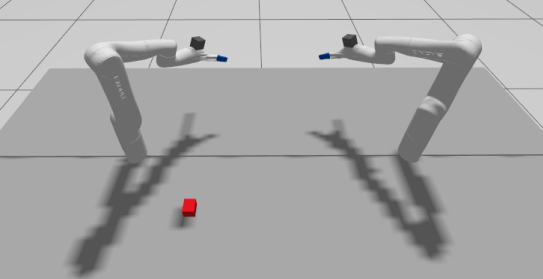
\includegraphics[width=0.7\linewidth]{Images/sharedVision/sim_setup.png}
\caption{Gazebo/ROS2 simulation setup: two Kinova Gen3 Lite arms sharing a tabletop workspace with a
fiducial target~\citep{sk2025sharedvision}.}
\label{fig:sv_simsetup}
\end{figure}

\begin{figure}[htbp]
\centering
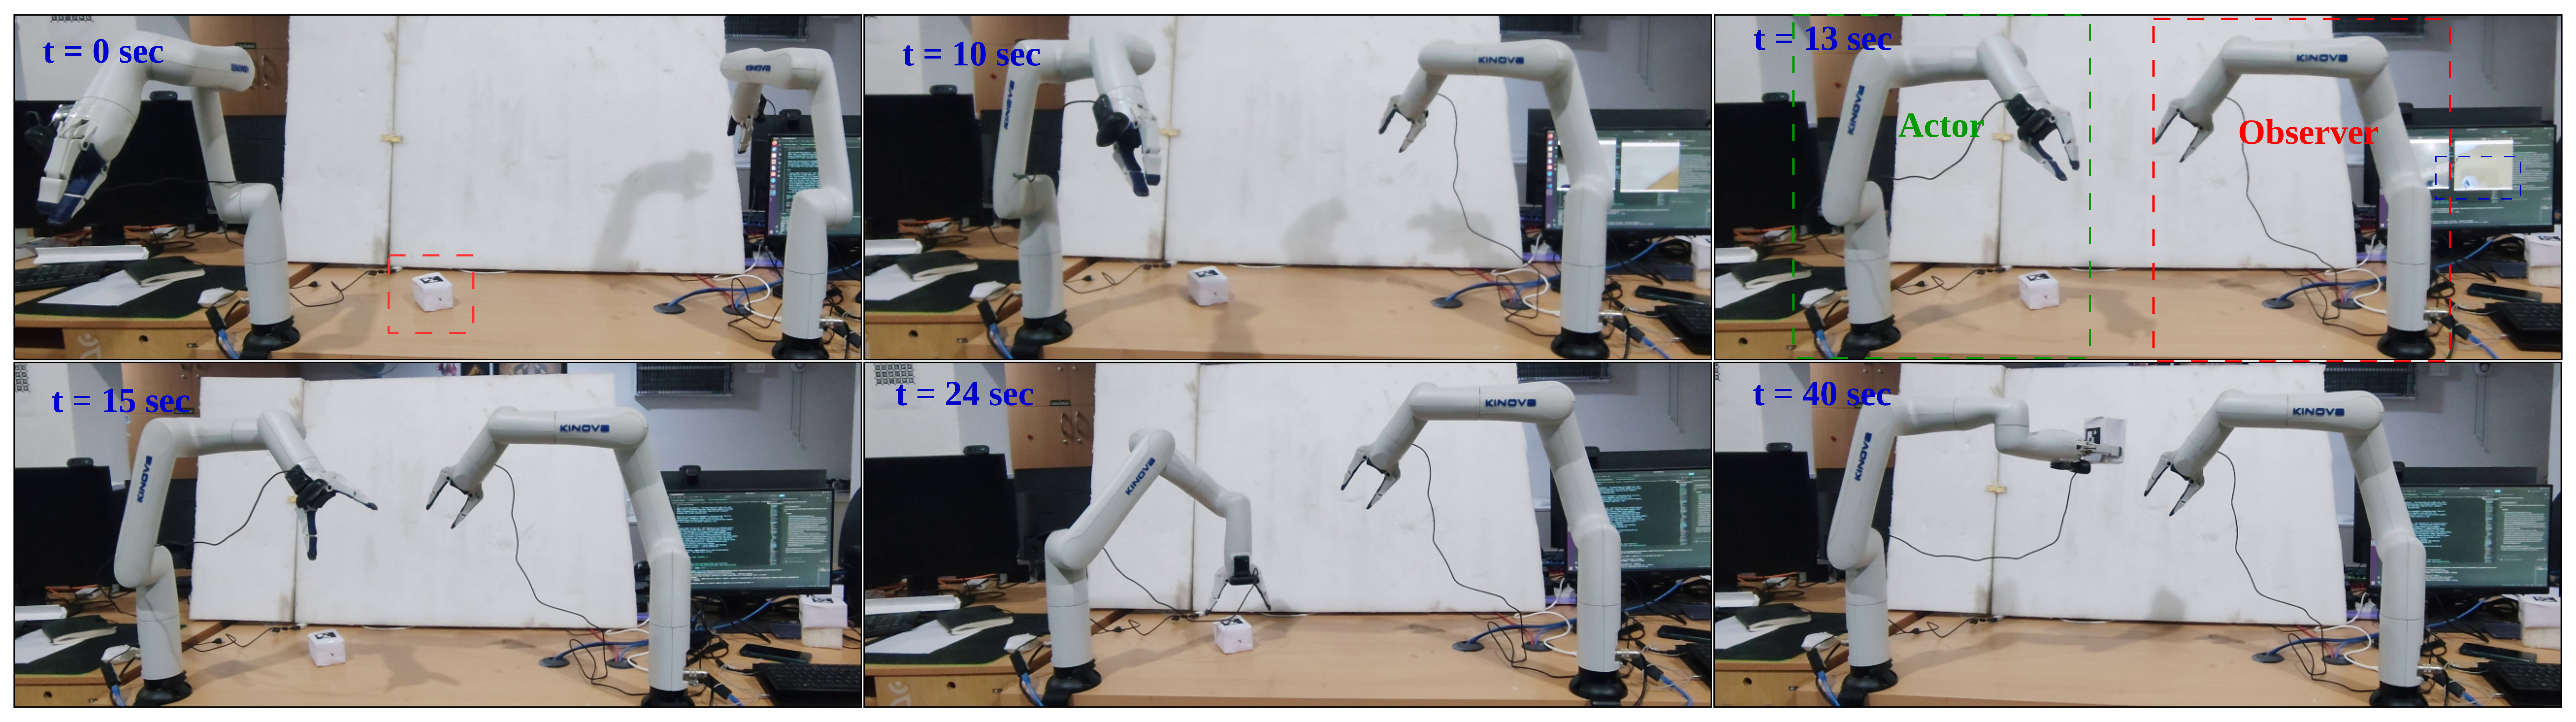
\includegraphics[width=\linewidth]{Images/sharedVision/hardware_experiment_left.jpg}
\caption{Experiment 1 (hardware): LEFT arm selected as actor, RIGHT arm idle. Frames show search,
detection, approach, grasp, and place~\citep{sk2025sharedvision}.}
\label{fig:sv_hwexp1}
\end{figure}

Two representative hardware trials illustrate the complete pipeline end-to-end: in Experiment 1 the
LEFT arm was selected as the acting arm (Figure~\ref{fig:sv_hwexp1}, Figure~\ref{fig:sv_lefttraj},
Figure~\ref{fig:sv_lefterror}), while in Experiment 2 the RIGHT arm was selected
(Figure~\ref{fig:sv_righttraj}, Figure~\ref{fig:sv_righterror}), with the non-selected arm remaining
idle in each case.

\begin{figure}[htbp]
\centering
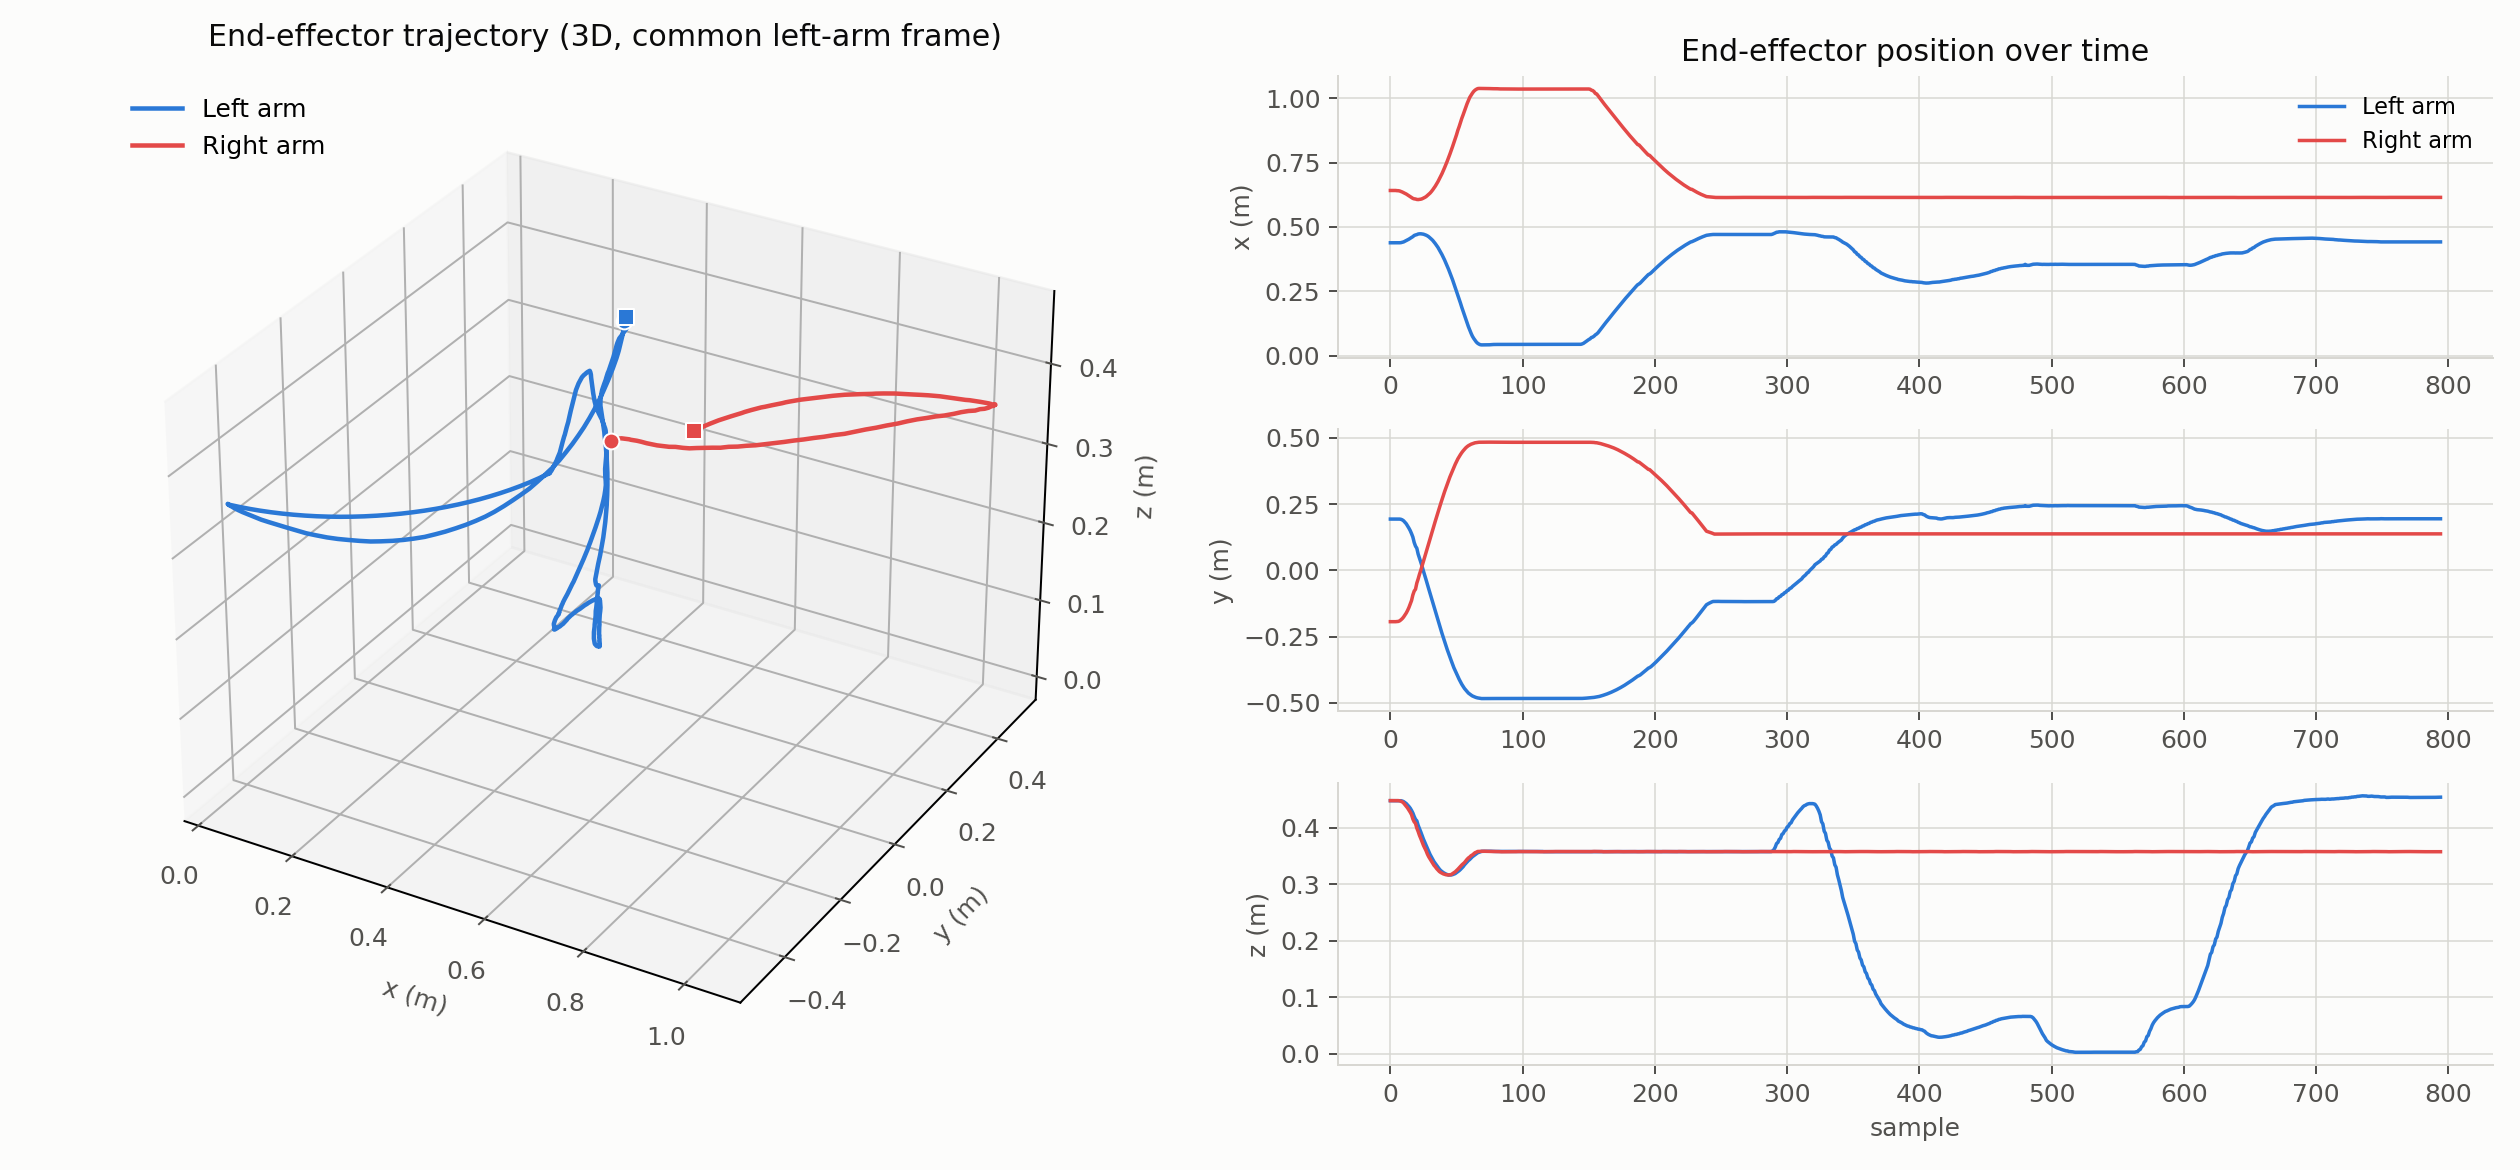
\includegraphics[width=\linewidth]{Images/sharedVision/end_effector_trajectories_left.png}
\caption{Experiment 1: end-effector trajectories in the common LEFT-arm frame (left) and per-axis
position over time (right). LEFT traces approach--descend--lift--place; RIGHT remains
stationary~\citep{sk2025sharedvision}.}
\label{fig:sv_lefttraj}
\end{figure}

\begin{figure}[htbp]
\centering
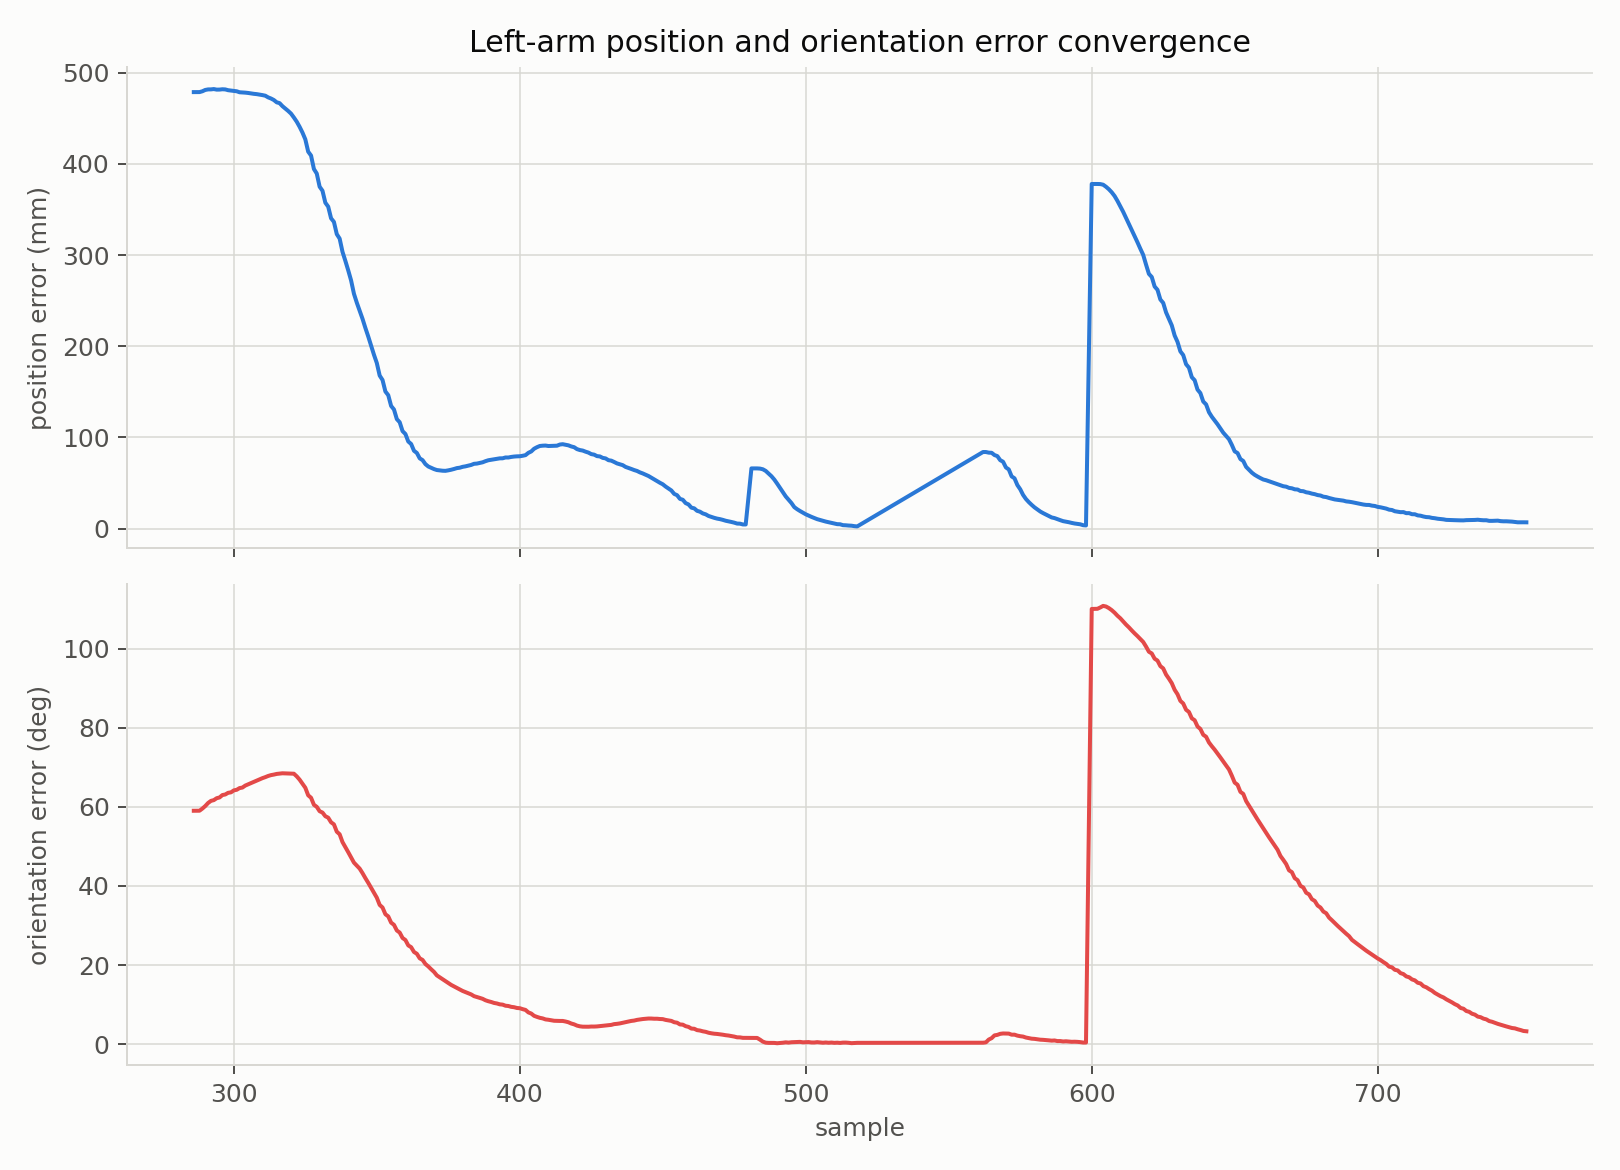
\includegraphics[width=0.7\linewidth]{Images/sharedVision/error_convergence_left.png}
\caption{Experiment 1: LEFT-arm position and orientation error, showing a convergence transient at
each waypoint transition~\citep{sk2025sharedvision}.}
\label{fig:sv_lefterror}
\end{figure}

\begin{figure}[htbp]
\centering
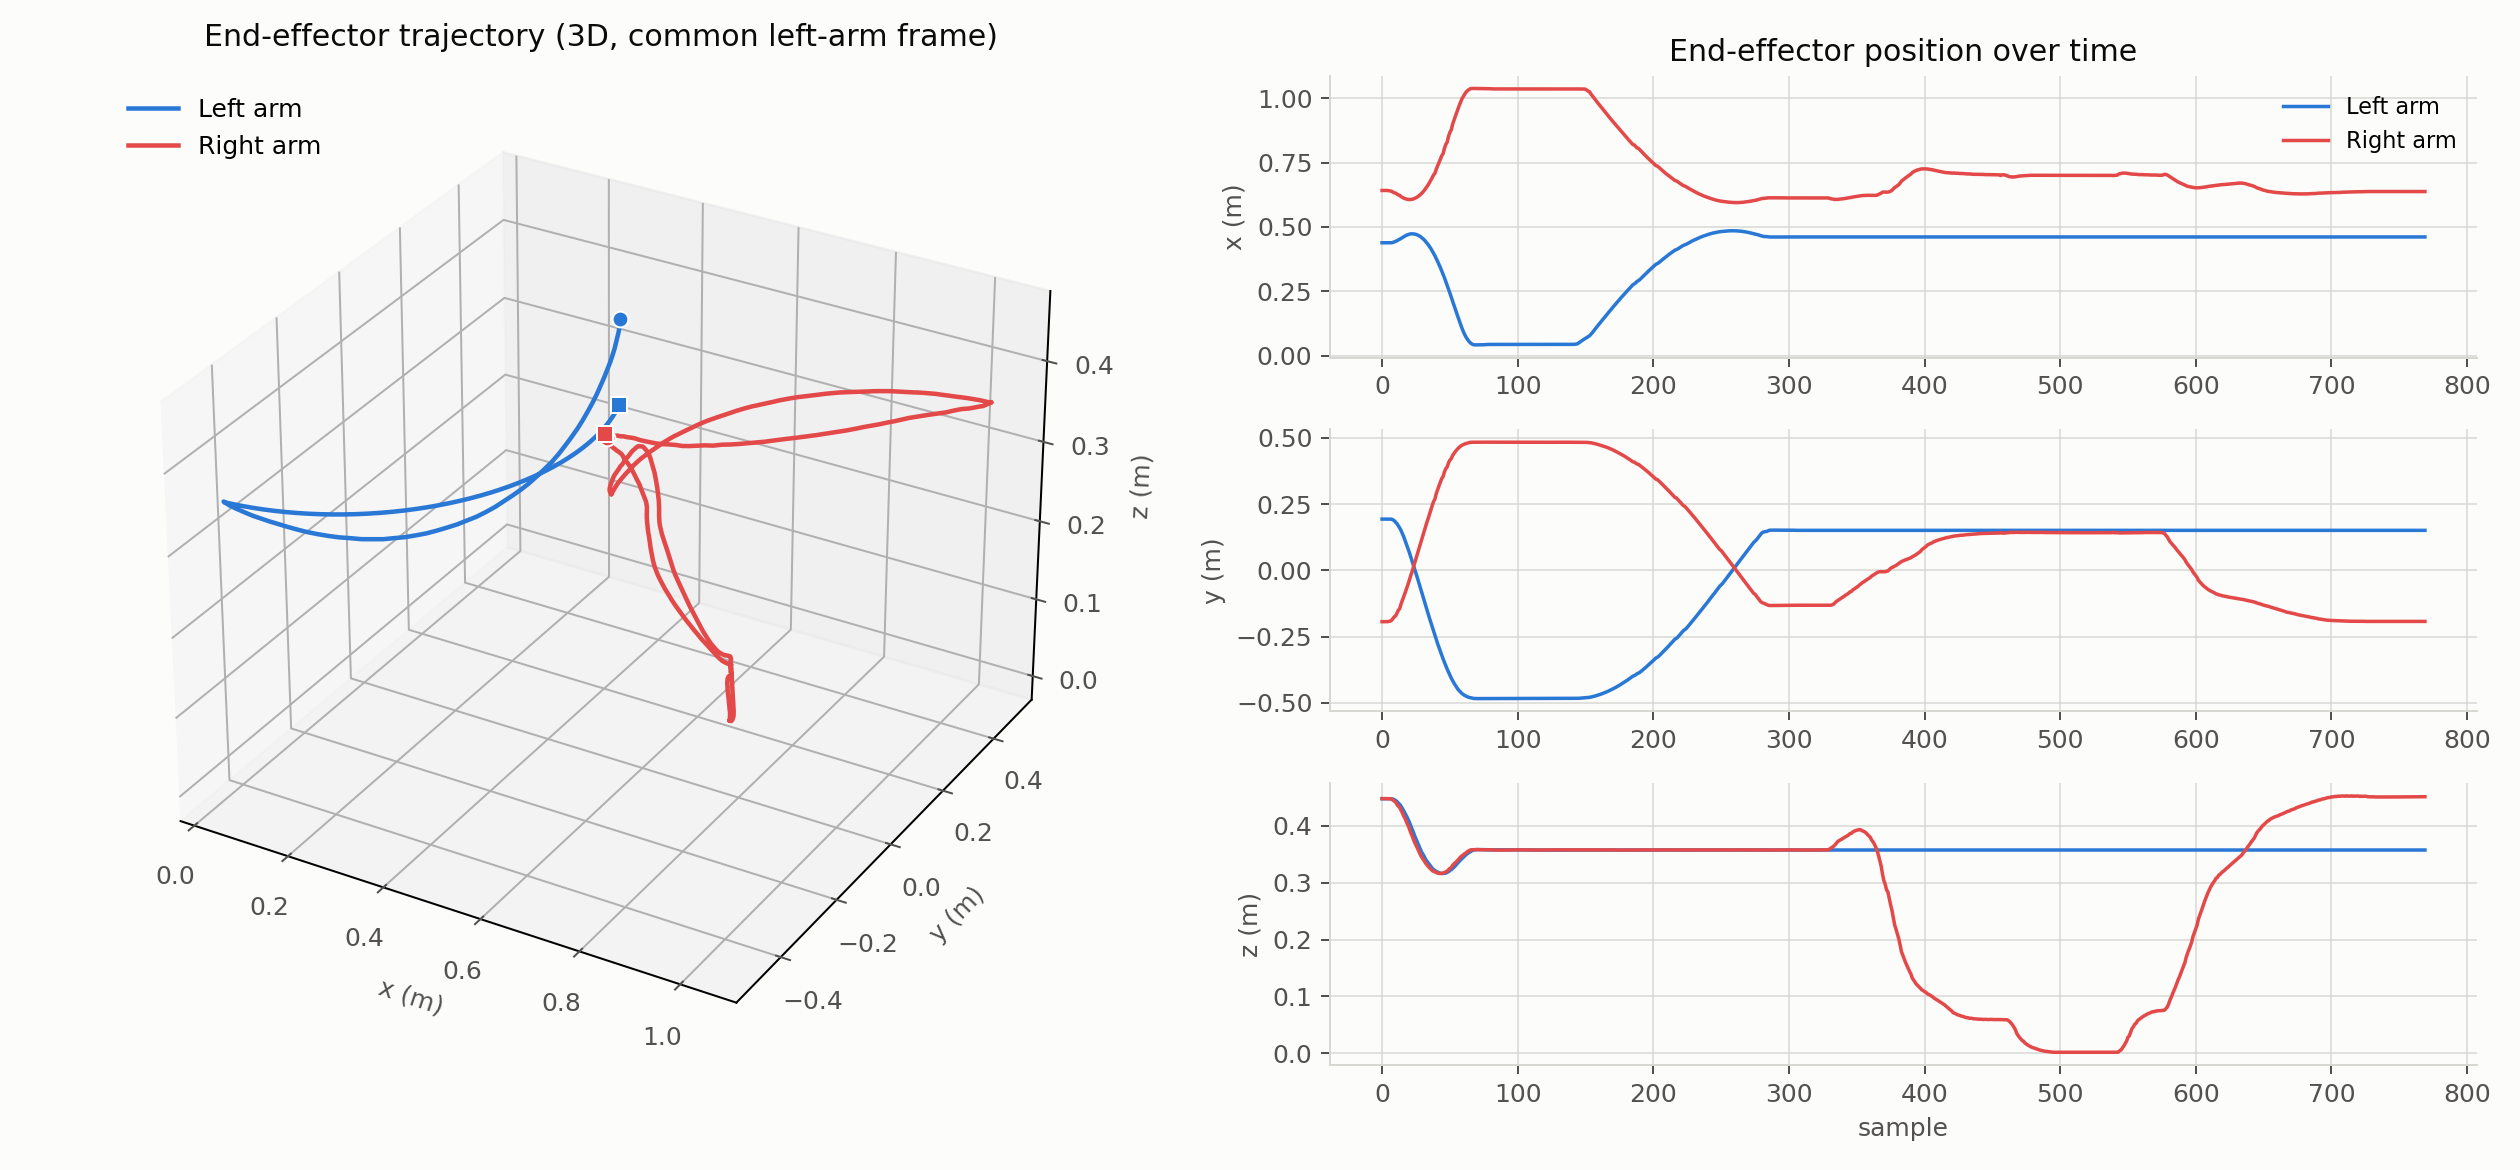
\includegraphics[width=\linewidth]{Images/sharedVision/end_effector_trajectories_right.png}
\caption{Experiment 2: end-effector trajectories and per-axis position with RIGHT selected as actor
and LEFT idle, the mirrored case of Figure~\ref{fig:sv_lefttraj}~\citep{sk2025sharedvision}.}
\label{fig:sv_righttraj}
\end{figure}

\begin{figure}[htbp]
\centering
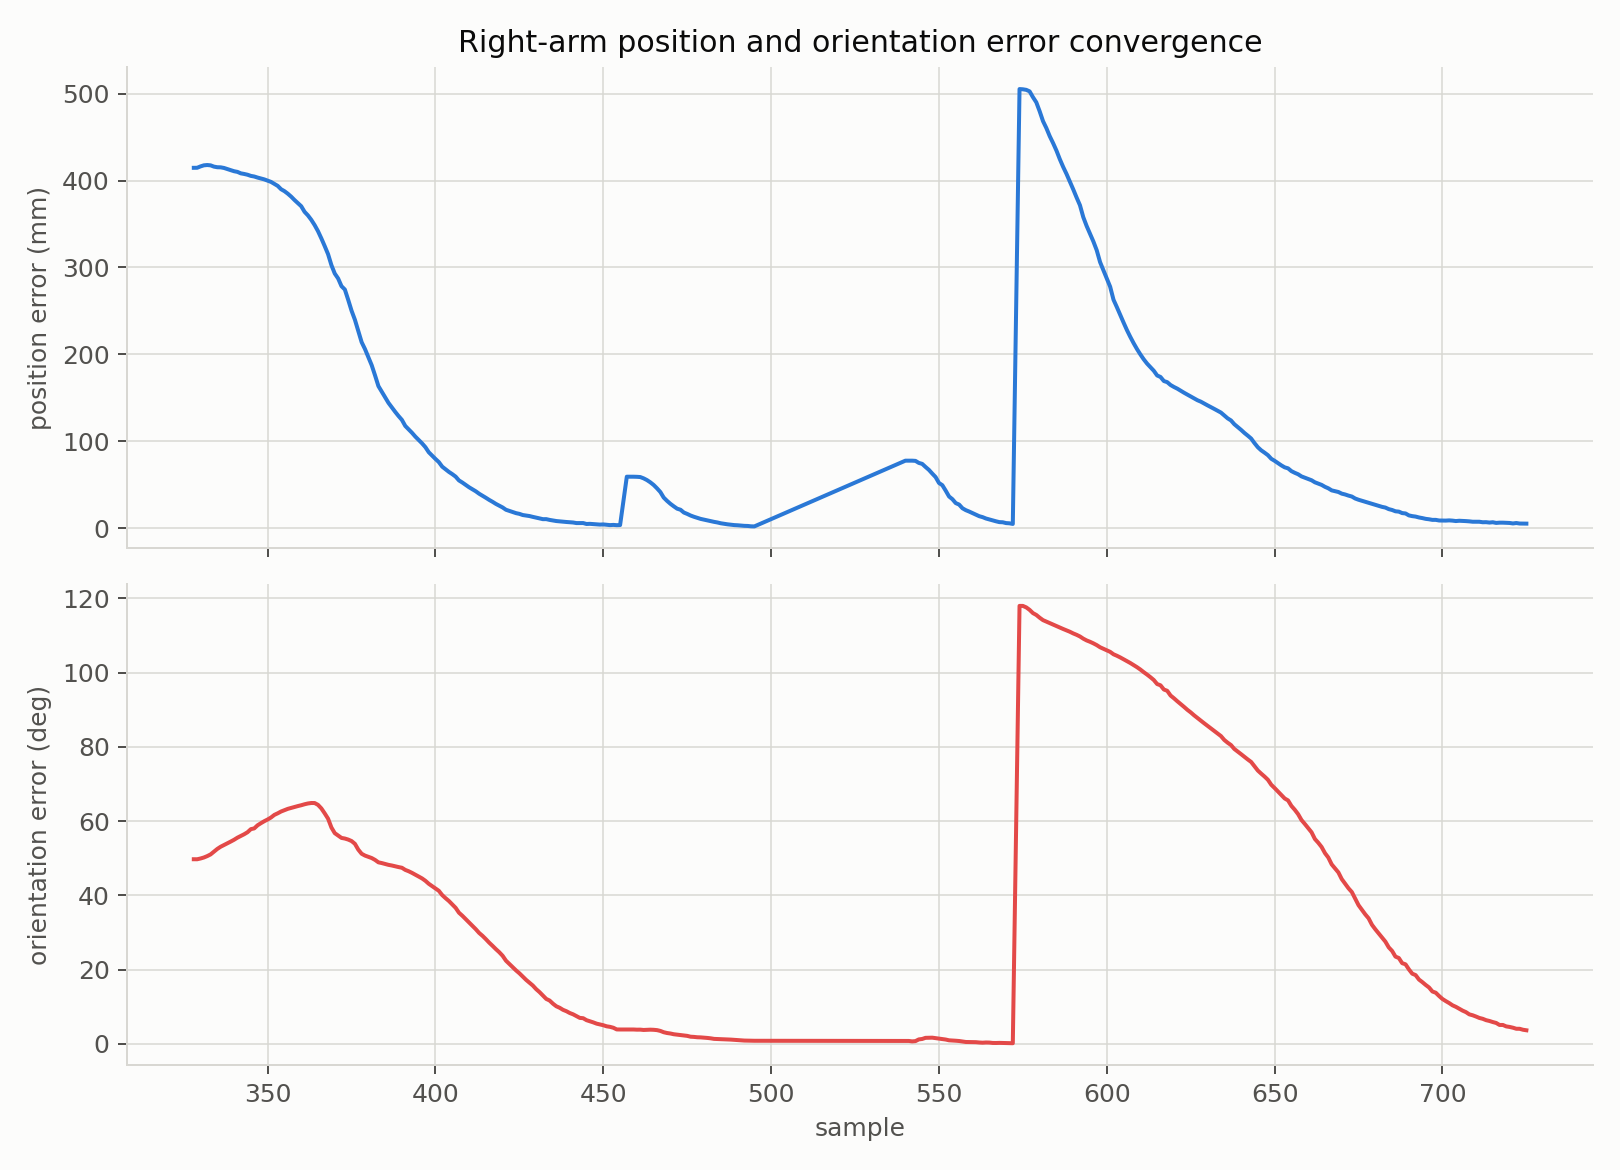
\includegraphics[width=0.7\linewidth]{Images/sharedVision/error_convergence_right.png}
\caption{Experiment 2: RIGHT-arm position and orientation error convergence~\citep{sk2025sharedvision}.}
\label{fig:sv_righterror}
\end{figure}

Figure~\ref{fig:sv_lefttraj} shows the LEFT arm's end effector tracing the full waypoint sequence,
approach, descend, lift, and place, while the RIGHT arm's position remains essentially flat across
the same sample range, consistent with it never receiving a motion command once the
reachability-based rule assigned the task to LEFT. The corresponding error convergence in
Figure~\ref{fig:sv_lefterror} shows the position and orientation error dropping from its initial
value toward zero, then rising again before converging a second time later in the sequence,
reflecting that each waypoint transition presents the resolved-rate controller with a fresh,
non-zero error that must be driven back down under Equation~\eqref{eq:sv_dls}, rather than the arm
tracking a single continuous trajectory. Figure~\ref{fig:sv_righttraj} and
Figure~\ref{fig:sv_righterror} show the mirrored case, with RIGHT selected as the acting arm and
LEFT idle; the same qualitative pattern holds, indicating that the pipeline behaves consistently
regardless of which arm the reachability rule selects.

\begin{table}[htbp]
\centering
\caption{Final position and orientation error at declared convergence, over five trials with each
arm selected as actor.}
\label{tab:sv_errormetrics}
\begin{tabular}{ccc}
\toprule
\multicolumn{3}{c}{\textbf{LEFT}} \\
\midrule
\textbf{Trial} & \textbf{Position error (mm)} & \textbf{Orientation error (deg)} \\
\midrule
1 & 2.549 & 0.310 \\
2 & 2.553 & 0.780 \\
3 & 4.587 & 0.053 \\
4 & 3.257 & 1.222 \\
5 & 2.818 & 0.715 \\
\textbf{Mean} & \textbf{3.153} & \textbf{0.616} \\
\textbf{Std. dev.} & \textbf{0.852} & \textbf{0.451} \\
\midrule
\multicolumn{3}{c}{\textbf{RIGHT}} \\
\midrule
\textbf{Trial} & \textbf{Position error (mm)} & \textbf{Orientation error (deg)} \\
\midrule
1 & 2.183 & 0.842 \\
2 & 2.640 & 0.767 \\
3 & 3.144 & 0.641 \\
4 & 2.447 & 1.023 \\
5 & 3.397 & 0.156 \\
\textbf{Mean} & \textbf{2.762} & \textbf{0.686} \\
\textbf{Std. dev.} & \textbf{0.500} & \textbf{0.327} \\
\bottomrule
\end{tabular}
\end{table}

Table~\ref{tab:sv_errormetrics} reports the position and orientation error at the point convergence
was declared, across five trials with LEFT selected as the acting arm and five trials with RIGHT
selected. Mean final position error was 3.153\,mm (LEFT) and 2.762\,mm (RIGHT), with orientation
error of $0.616^\circ$ (LEFT) and $0.686^\circ$ (RIGHT); standard deviations remained under 1\,mm
and under $0.5^\circ$ in both cases. These figures indicate that the resolved-rate control loop of
Section~\ref{subsec:sv_dls} consistently reaches sub-5\,mm, sub-$1.3^\circ$ final accuracy
independent of which arm is assigned the task, suggesting no meaningful asymmetry between the two
arms' manipulation precision despite their different mounting positions and per-arm approach
offsets. Consistent with the proof-of-concept scope of this validation, these five trials per arm
establish repeatability rather than a fully powered statistical characterization of the system, and
the reachability test of Equation~\eqref{eq:sv_reach} is a simple axis-aligned workspace box rather
than a full manipulability or collision-aware reachability model; both are natural directions for
future extensions of this work.

The dual-arm shared-vision system developed in this chapter answers \emph{which} arm should act on
a jointly visible target, evaluated once at the moment of detection. It does not yet address whether
the two arms, now sharing a workspace and free to move concurrently rather than one at a time, can
collide with one another during that concurrent motion. Chapter 5 takes up exactly that question,
addressing gap G3 with a kinematics-based framework for real-time inter-arm distance monitoring.
